\chapter{Results and Discussions}
\label{cha:results}

\section{Users' gender}
\label{sec:resusergender}
We retrieved information about a user gender in two ways: UsersBoxes and User’s settings. These data were then used to categories users’ in groups.

\subsection{UserBoxes}
\label{sec:resuserboxes}
Analyzing UserBoxes we retrieve relatively few data. Most Wikipedia users do not spend much time on their user page. To insert a UserBox it is required an effort by the user, that most are not willing to take. Gender UserBoxes allow a wide personalization and more can be added as needed. All genders are macro-categorized as Masculine, Feminine, Non-Binary and Other. 

\begin{table}[H]
    \centering
    \ra{1.2}
    \begin{tabularx}{\columnwidth}{@{}Xr@{}}
        \midrule
        \textbf{Genders categories} & \textbf{Number of users that used one of those UserBox} \\ \toprule
        Masculine & 10,489 Users  \\
        Feminine &  2,045 Users \\
        Non-Binary &  347 Users \\
        Other &  218 Users \\
        \bottomrule
        Total &  13,099 Users \\

         \bottomrule
    \end{tabularx}
    
    \caption{The table shows the number of users that implemented a UserBox of a particular category. \label{table:datasetsize}}
\end{table}

This approach may be subjected to some biases. Users that do not feel included in the limited gender selection of the Wikipedia user profile, may tend to express their identity through this feature, while users correctly represented on their settings, may not feel the need to use this feature. Another known bias, particularly on internet community, is the tendency, from female users, to not specify their gender or specify it as male. This is due to the fact that female users are subjected to discrimination in these platforms and tend to hide their true gender.

\begin{figure}[H]
    \centering
    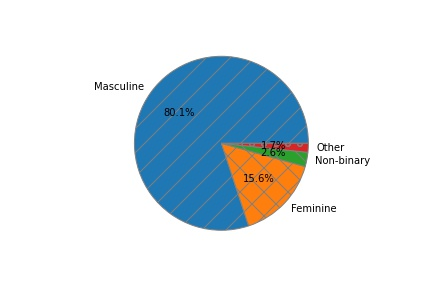
\includegraphics[width=0.6\textwidth]{./img/userbox.jpg}
    \caption{Percentage of editors with a UserBox for each gender group}
    \label{fig:userbox}
\end{figure}

We choose to not use this data, because it was statistically too small if compared to the profile settings and would generate groups to with few to no data at all.

\subsection{Profile settings}
\label{sec:resprofilesettings}
Profile settings is the most used feature to express a user gender. Its options are limited to male, female and unknown, where the unknown option is set by default. Most users never change this option, and are thus categorized as unknown, so, this specific label does not represent any valuable information.

This information is subjected to the same biases stated above, but it was the best we could do with the resources we had. Our results show a similar distribution of female and man to more accurate studies such as "Gender differences in Wikipedia editing" \cite{antin2011gender}. We can confidently say our results are a good representation of male and female users in Wikipedia.

We only needed data about English, Spanish, Italian and Catalan Wikipedias, but we decided to collect data for all Wikipedias. The results for the most common Wikipedia languages are shown in table 4.2.

\begin{table}[H]
    \centering
    \ra{1.2}
    \begin{tabularx}{\columnwidth}{@{}Xrrr@{}}
        \midrule
        \textbf{Wikipedia} & \textbf{Female Users} & \textbf{Male Users} & \textbf{All Users} \\ \toprule
        English & 122,445 & 604,633 & 40,526,936  \\
        Spanish & 30,774 & 106,269 & 6,071,869  \\
        German & 14,371 & 79,010 & 3,603,382 \\
        French & 9,275 & 48,531 & 3,968,600 \\
        Russian & 55,065 & 173,019 & 2,891,204 \\
        Italian & 7,731 & 39,037 & 2,060,494  \\
        Catalan & 1,499 & 5,145 & 373,672  \\

         \bottomrule
    \end{tabularx}
    
    \caption{The table shows the number female, male and total user for the most used Wikipedia. \label{table:datasetsize}}
\end{table}

This data was used in to generate two user groups: female and male.

We analyzed the gender distribution for users with different edits counts, since it is a simple way to identify a user level of activities, and it can be said that users with more edits are more active. The results are shown in Figure 4.2.

\begin{figure}[H]
    \centering
    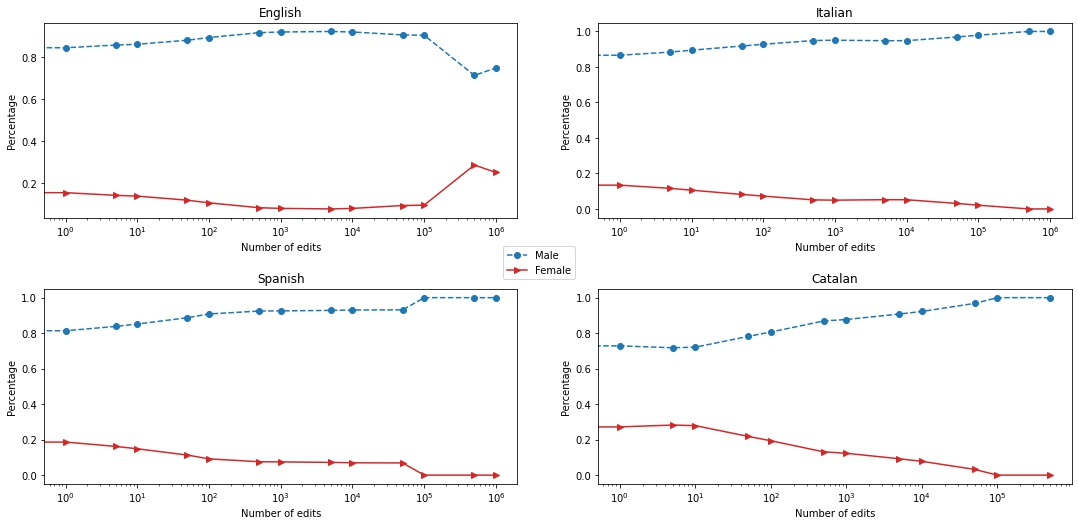
\includegraphics[width=0.95\textwidth]{./img/gedit.jpg}
    \caption{Percentage of male and female based on edit count, in four different Wikipedia. The users edit count is calculated based on a series of threshold, that a user can reach. The thresholds are: $0, 1, 5, 10, 50, 10^2, 5 \cdot 10^2, 10^3, 5 \cdot 10^3, 10^4, 5 \cdot 10^4, 10^5, 5 \cdot 10^5, 10^6$  }
    \label{fig:gedit}
\end{figure}

Our analysis compares male users and female users to a reference made by all users. All data have been shared in our group, but it was not made publicly available to avoid users’ privacy violations.

As seen in Figure \ref{fig:gedit} male editors are the vast majority of users, and the difference between male and female editors tend to grow with the edit count.


\section{Emotions}
\label{sec:resemotions}
Emotions are the core of this study. We analyzed the emotion expressed by users on the article and user talk pages. The analysis was done with EmoLex.

\begin{table}[H]
    \centering
    \ra{1.2}
    \begin{tabularx}{\columnwidth}{@{}Xrrr@{}}
        \midrule
        \textbf{WikiConv} & \textbf{Action analyzed} & \textbf{Words analyzed} \\ \toprule
        English & 4,163,088 & 1,178,703,180 \\
        Spanish & 469,051 & 95,987,997 \\
        Italian & 245,886 & 45,248,302 \\
        Catalan & 28,557 & 7,264,086 \\
         \bottomrule
    \end{tabularx}
    
    \caption{The table shows the number of actions and words analyzed foreach WikiConv Dataset during our analysis. \label{table:datasetsize}}
\end{table}

Our first result was to calculate how much each emotions was expressed in the language we analyzed. We estimated the percentage of words which express an emotion or a sentiment over all words analyzed that were contained in the emotion dictionary. The results are shown in Figure \ref{fig:emlang}.

\begin{figure}[H]
    \centering
    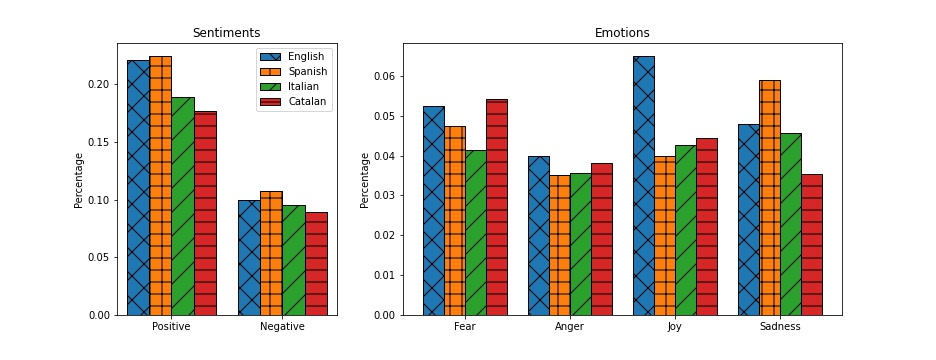
\includegraphics[width=0.95\textwidth]{./img/emlang.jpg}
    \caption{ The tables shows the percentage of emotions and sentiment expressed in all talk pages on different Wikipedia }
    \label{fig:emlang}
\end{figure}

\subsection{Word Clouds}
We analyzed a great quantity of data. It was necessary to have a visual representation of what we were doing. We choose to represents the most common words identified as emotions by our dictionaries in a "Word Cloud".\footnote{\url{https://amueller.github.io/word_cloud/}} Some sample results can be seen in Figure

\begin{figure}[H]
    \centering
    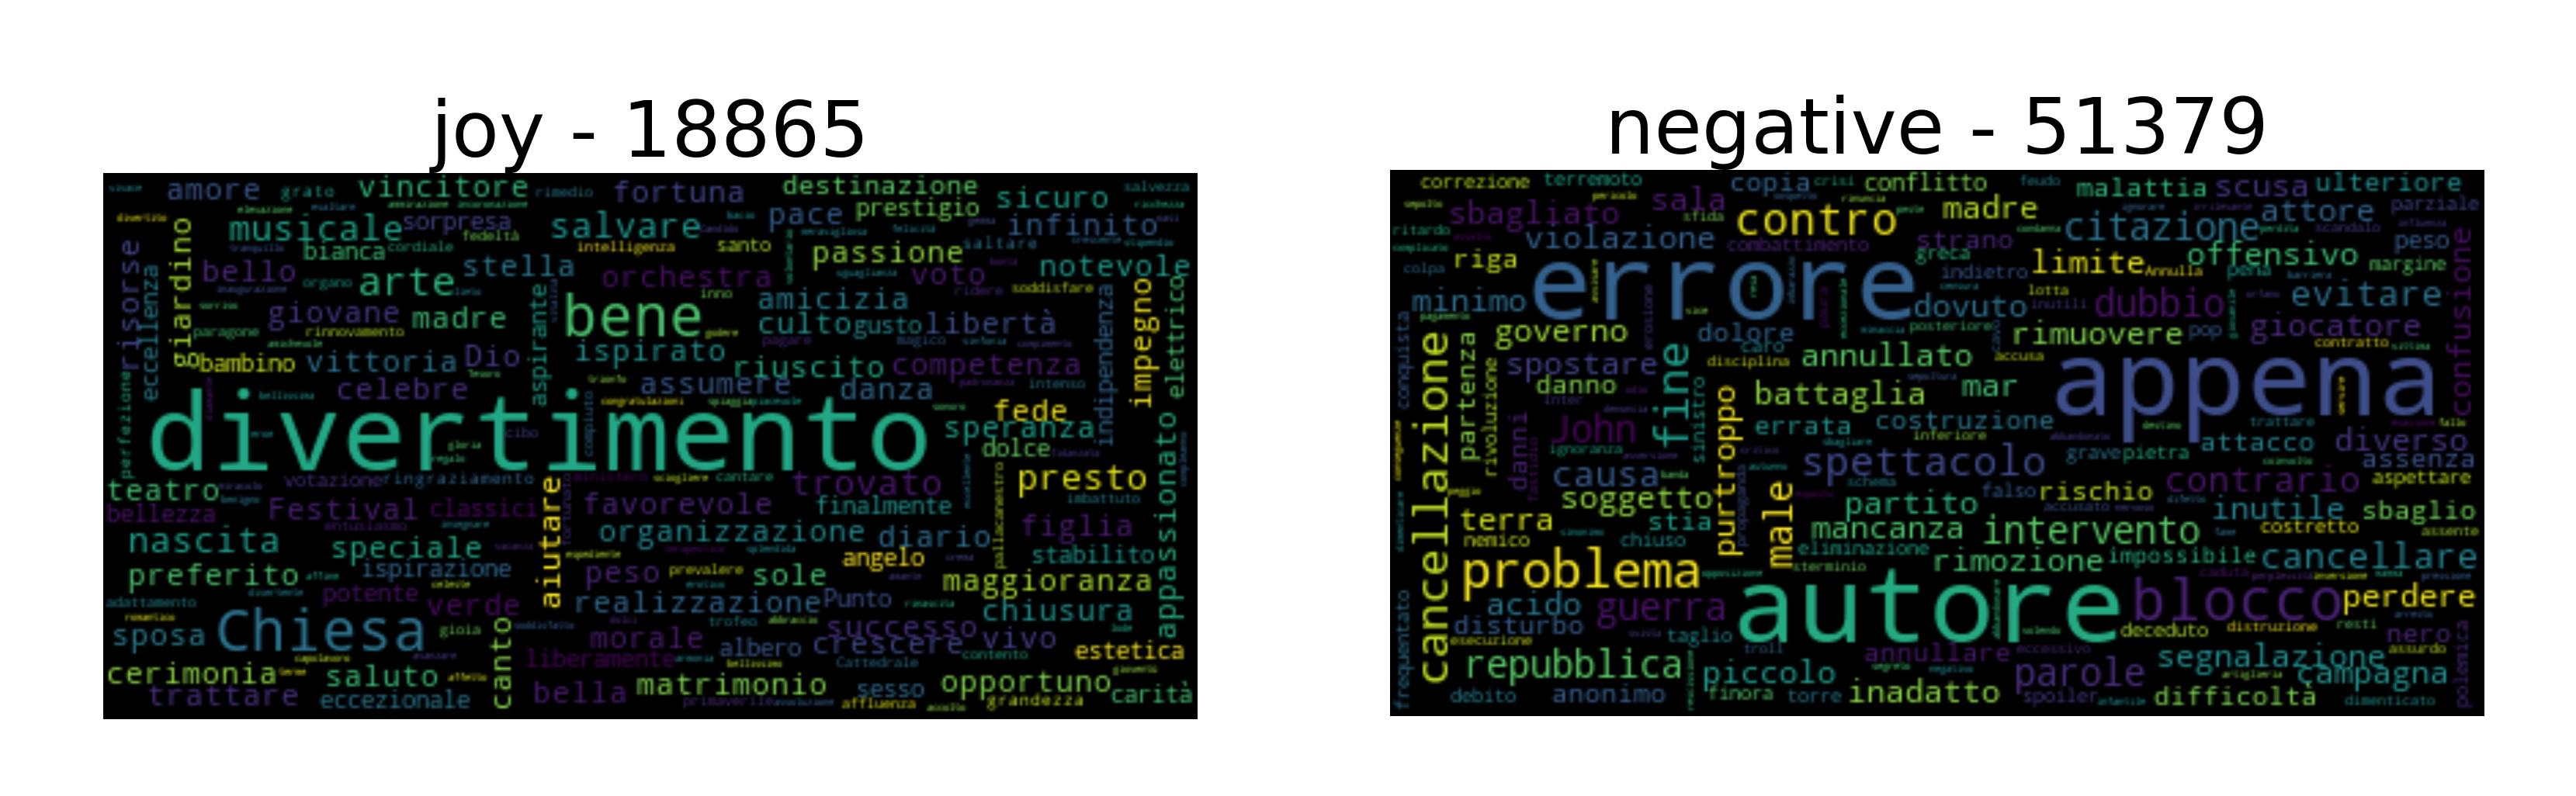
\includegraphics[width=0.95\textwidth]{./img/cloud.png}
    \caption{ This are two example of "Word Clouds" extracted from the Italian WikiConv of November 2019. The dimensions of a word in these images is directly related to their presence in the dataset. The number on the title is the total number of analyzed words that belong to that particular emotions. }
    \label{fig:cloud}
\end{figure}


\subsection{Users}
\label{sec:resusers}
We can use users' group previously defined to analyze their different emotional response. For each user we calculate the average value for the emotions over all its actions and averaged this with all other users in a group. The results can be seen in Figure \ref{fig:emgender} and Figure \ref{fig:emroles}.

\begin{figure}[H]
    \centering
    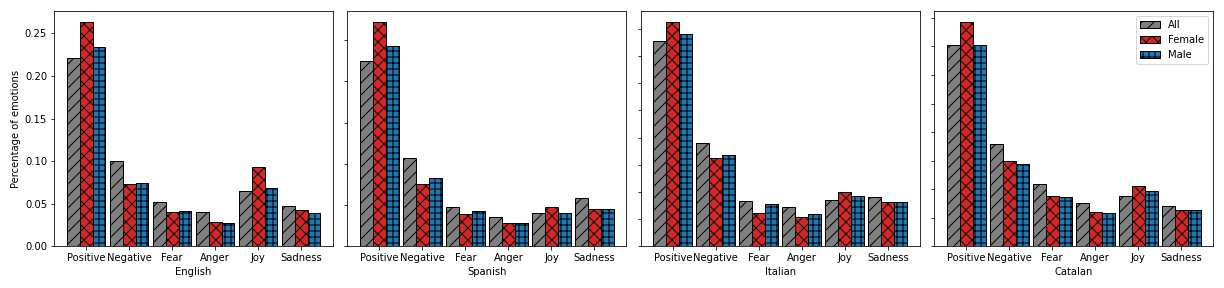
\includegraphics[width=0.95\textwidth]{./img/emgender.jpg}
    \caption{ The tables shows the percentage of emotions and sentiment expressed by female, male or all users }
    \label{fig:emgender}
\end{figure}

\begin{figure}[H]
    \centering
    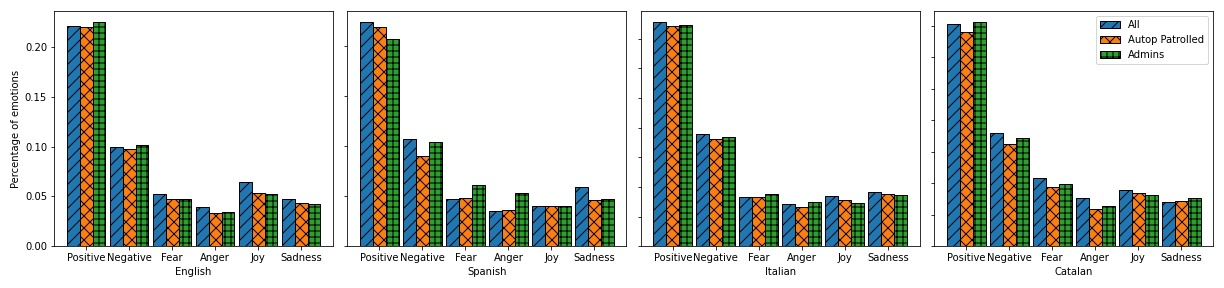
\includegraphics[width=0.95\textwidth]{./img/emroles.jpg}
    \caption{ The tables shows the percentage of emotions and sentiment expressed by admins, auto patrolled and for all user }
    \label{fig:emroles}
\end{figure}

In figure \ref{fig:emgender} we can see that female editor have a tendency to express more positive sentiment than male. This is was also show in previous studies \cite{laniado2012emotions} \cite{iosub2014emotions}.

We are interested in users life-cycles, from when they join Wikipedia to the moment they leave. To better understand how users feels during their life as a Wikipedia editor we analyzed all emotions they express. We took an average of a user action in each month after their complete their first action, and averaged them with all users in a group or with all Wikipedia's users. We took into consideration that the number of active users decrees over time. We also analyzed the emotions a user received from others.

\begin{figure}[H]
    \centering
    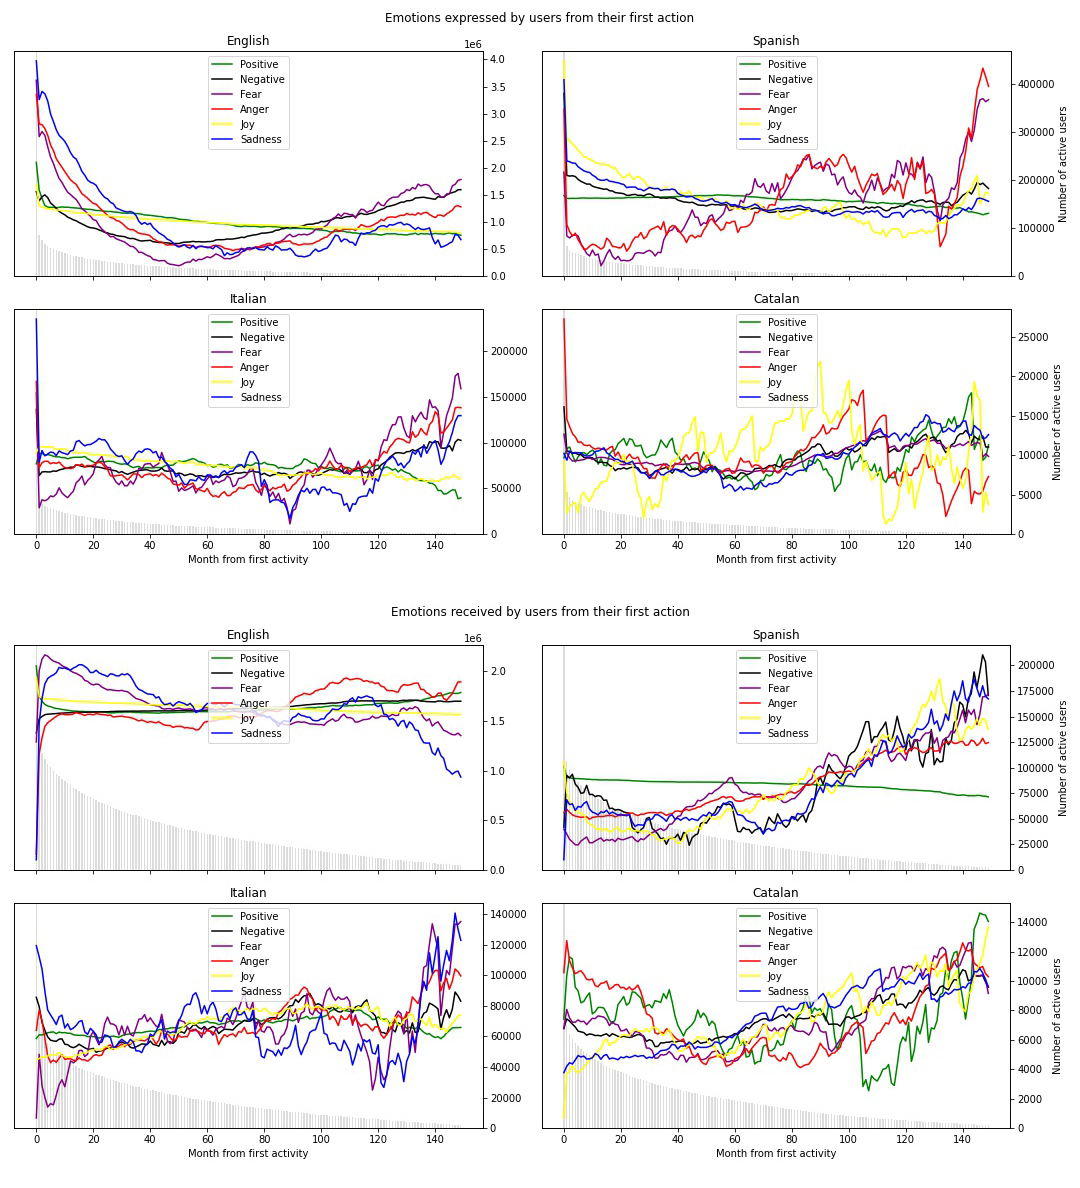
\includegraphics[width=1\textwidth]{./img/mstart.jpg}
    \caption{ The two tables shows the normalized value of each emotion and sentiment analyzed for four languages.  The bars in the background represent the number of active users it and the x axis are the month from a user first activity. The first table shows the emotions expressed by a users in they actions and the second the emotions received through reply to their posts. }
    \label{fig:mstart}
\end{figure}

Life-cycles can also be analyzed for different users' groups and compared between them. This can be useful to understand differences between different users.

\begin{figure}[H]
    \centering
    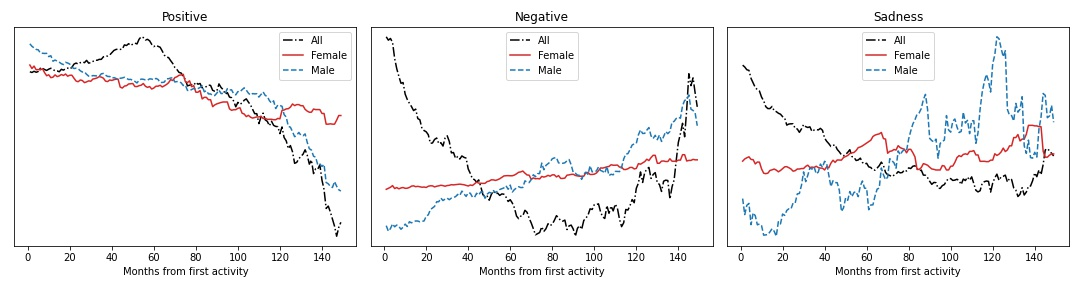
\includegraphics[width=0.9\textwidth]{./img/gtime.jpg}
    \caption{ The two tables shows the normalized value of different positive, negative and sad words used by users of different gender from their first action. }
    \label{fig:gtime}
\end{figure}

To understand how external events influence users on Wikipedia it is useful to see variation of emotions over time. For this reason we analyzed user emotions for over each month from the opening of Wikipedia, in a similar way we analyzed user life-cycle. It is important to remember that, in the early days Wikipedia was less used, and we have less data. Wikipedia reached a good level of popularity around 2007.

\begin{figure}[H]
    \centering
    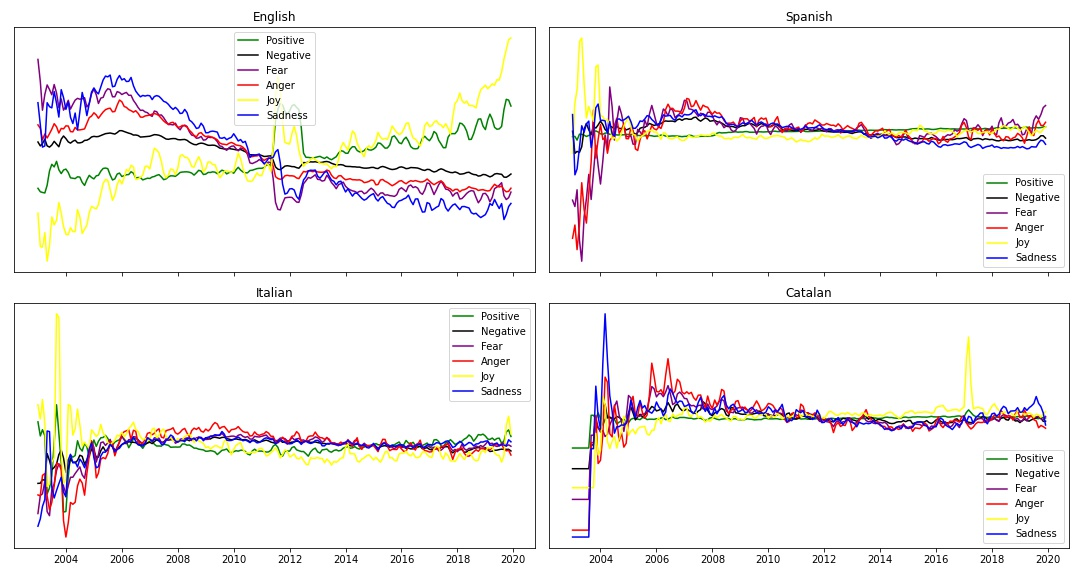
\includegraphics[width=0.9\textwidth]{./img/time.jpg}
    \caption{ The table shows the normalized value of all analyzed emotions over time. The emotions are sampled each month }
    \label{fig:time}
\end{figure}

\subsection{Pages}
\label{sec:respages}
Pages were analyzed similarly to users. In this case there were less privacy concerns since pages aggregate contribution from different users. We did not made any groups of pages. Smaller pages do not have enough information to be considered statistically useful, but bigger pages could be analyzed. Since it did not increase significantly our calculation time, we decided to analyze all pages and save the metrics we generated to our database.

Every page has a metric for each emotion and sentiment from any month of its life.

\begin{figure}[H]
    \centering
    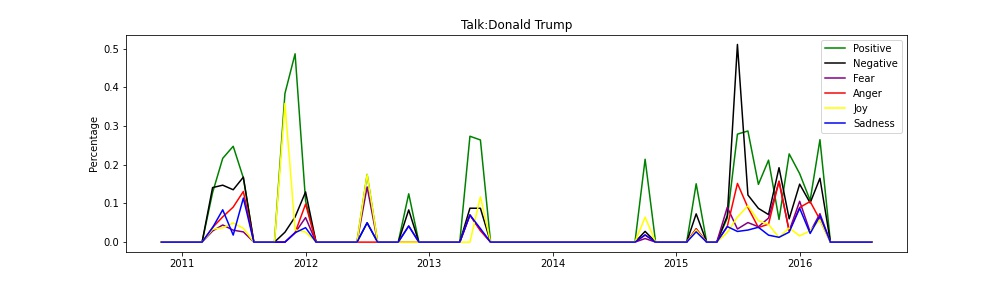
\includegraphics[width=1\textwidth]{./img/trump.jpg}
    \caption{ The table shows the emotions expressed by editors on the talk page of the article related to Donald J. Trump }
    \label{fig:trump}
\end{figure}
